% !TEX root = ../dsv_script.tex
%
Eine Grundvoraussetzung f\"ur eine praktisch n\"utzliche digitale Signalverarbeitung ist die M\"oglichkeit zwischen dem analogen und digitalen Bereich wechseln zu k\"onnen. Hierbei sollte man auch genau quantifizieren k\"onnen, ob bei diesem Prozess Informationen verloren gehen, oder wie man garantieren kann, dass diese Umwandlung verlustfrei vonstatten geht. Meist nutzt man hierf\"ur das Nyquist-Shannon Sampling Theorem~\cite[Kapitel~1.4.2]{proakis2013}. Die hieraus resultierende sogenannte Nyquist-Sampling-Theorie fu{\ss}t bekannterma{\ss}en auf der Repr\"asentation von bandbegrenzten Signalen durch hinreichend dichte \"aquidistante Abtastwerte. Diese Theorie ist gut studiert, in Textb\"uchern aufbereitet und bildet die Grundlage f\"ur viele Messsysteme und Algorithmen im Digitalen, siehe beispielsweise~\cref{dftintp}.

Es gibt jedoch auch einige Nachteile von Nyquist-Sampling, die aus dessen Annahmen und der daraus folgenden Verarbeitung entstehen. Einerseits kann ein endliches Signal im Allgemeinen \emph{nicht} bandbegrenzt sein. Weiterhin entstehen durch die Bandlimitierung von Signalen Gibbs-Artefakte, die besonders in Bildern nicht erw\"unscht sind. Geht es um die Auswertung $x(t)$ eines Signals $x$ zwischen den aufgenommenen Samples $x[n]$, also Interpolation, hat man das Problem, dass die $\Sinc$-Funktion nur sehr langsam mit Rate $1/t$ abf\"allt. Diese Eigenschaft f\"uhrt dazu, dass man f\"ur die Bestimmung eines Wertes $x(t)$ mit einer Genauigkeit von \SI{1}{\percent} etwa $100$ um $t$ benachbarte Samples betrachten muss. Das hei{\ss}t, vor allem bei 2D-Interpolation skaliert der resultierende Rechenaufwand nicht sehr g\"unstig, falls hohe Genauigkeit ben\"otigt wird.

Aus diesem Grund m\"ochten wir uns eine alternative Sampling-Theorie genauer ansehen -- die B-Splines~\cite{unser1999splines_mag}. Wir f\"uhren zun\"achst die auf Polynomen basierende Signalverarbeitung ein und vergleichen sie anschlie{\ss}end zur bereits bekannten Nyquist-Theorie.

\subsubsection{B-Splines als Polynome}

Allgemein bezeichnet man st\"uckweise definierte und stetig differenzierbare Polynome als Splines. Man bezeichnet die Stellen an denen zwei unterschiedliche Polynome zusammensto{\ss}en als Knoten. Ein Spline der Ordnung $\ell \in \N$ ist ein Polynom vom Grad $\ell$, ist also von der Form
\begin{equation}
    p(x) = 
        a_{\ell} t^{\ell} 
        + a_{\ell - 1} t^{\ell-1} 
        + \dots
        + a_1 t 
        + a_{0}.
\end{equation}
%
Ein Spline ist nun eine Funktion $s(t)$, welche f\"ur Knoten $n = 1, 2, \dots$ definiert ist durch
\begin{equation}
    s(t) = \begin{cases}
        p_1(t) \fuer x \in [1,2], \\
        p_2(t) \fuer x \in [2,3], \\
        \vdots
    \end{cases}
\end{equation}
wobei sich die Glattheit durch die Forderung ergibt, dass die Funktion und ihre Ableitungen an den Knoten stetig sei, also
\begin{equation}
    \lim\limits_{t \rightarrow n^-} s^{(m)}(t) =
    \lim\limits_{t \rightarrow n^+} s^{(m)}(t)
\end{equation}
erf\"ullt ist, wobei $s^{(m)}$ f\"ur $m \geqslant 0$ die $m$-te Ableitung des Splines $s$ repr\"asentiert. In einer Arbeit~\cite{schoenberg1988bsplines}, die sogar dem ber\"uhmten Paper von Shannon vorausgeht, beschreibt Schoenberg, dass sich diese Splines der Ordnung $\ell$ via
\begin{equation}\label{bsplines_summation}
    s(t) = \Sum{k \in \Z}{}{
        c[k] \beta^{\ell}(t - k)
    }
\end{equation}
darstellen lassen. Hierbei ist die Funktion $\beta^\ell: \R \rightarrow \R$ definiert als eine iterierte Faltung einer Rechteck-Funktion via
\begin{equation}
    \beta^\ell = \underbrace{
        \beta^0 \ast \dots \ast \beta^0
    }_{(\ell+1) \Text{mal}}, 
    \Text{wobei}
    \beta^0(t) = \begin{cases}
        1,\quad \Abs{t} < \frac{1}{2} \\
        \frac{1}{2}, \quad \Abs{t} = \frac{1}{2} \\
        0, \Text{sonst.}
    \end{cases}
\end{equation}
In \cref{bsplines_all_splines} sind die Funktionen $\beta^\ell$ f\"ur $\ell = 0, \dots, 3$ dargestellt. Man erkennt sehr gut, dass der Grad der Glattheit von der Ordnung des Splines abh\"angt und dass die Funktionswerte $\beta^\ell(t)$ f\"ur $\Abs{t}>\ell+1/2$ verschwinden. Man spricht von Funktionen mit kompaktem Tr\"ager. Das hei{\ss}t die Summation in \eqref{bsplines_summation} ist f\"ur fixes $t \in \R$ \emph{endlich} und ist auf $\ell+1$ Summanden beschr\"ankt!
%
\begin{figure}
    \centering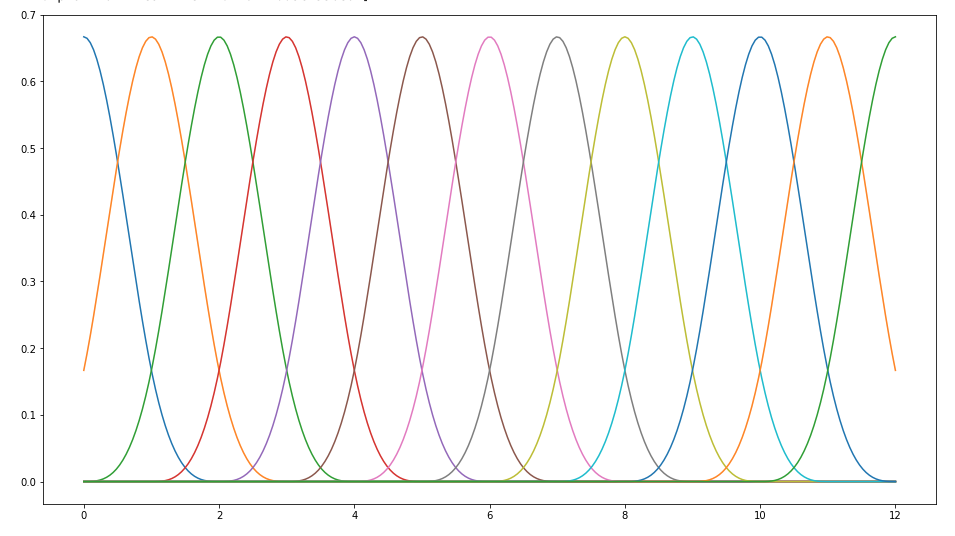
\includegraphics[width=0.9\textwidth]{img/bsplines/all_splines.png}
    \caption{Kubische B-Splines f\"ur Abtastung an den Werten $n = 0, \dots, 12$.}\label{bsplines_all_splines}
\end{figure}
%
Wir wollen nun eine explizite Formel f\"ur $\beta^\ell$ entwickeln. Hierzu betrachten wir die Fourier-Transformation 
\begin{equation}
    B^\ell(\omega) 
        = \left(\frac{\sin(\omega / 2)}{(\omega / 2)}\right)^{\ell + 1}
        = \frac{(\exp(\jmath \omega/2) - \exp(-\jmath \omega/2))^{\ell+1}}{
            (\jmath \omega)^{\ell + 1}
        }
\end{equation}
mit einigen Rechentricks (siehe \cite[Box 1.]{unser1999splines_mag}) kann man dies so lange umformen, bis man
\begin{equation}
    \beta^\ell(t) = \frac{1}{\ell !}\Sum{p = 0}{\ell+1}{
            \binom{\ell+1}{p}(-1)^p
            \left(t - p + \frac{\ell+1}{2}\right)_+^\ell
        }
    \Text{mit}
    (x)_+ = \begin{cases}
      x, \fuer x \geqslant 0, \\
      0, \Text{sonst},  
    \end{cases}
\end{equation}
erh\"alt. Damit ist $\beta^\ell$ wirklich ein Polynom $\ell$-ten Grades. Die Stetig- und Differenzierbarkeit muss man sich aber noch separat \"uberlegen. 

Weiterhin kann man zeigen, dass folgende Formeln f\"ur Differentiation und Integration von B-Splines gelten:
\begin{equation}\label{bsplines_deriv_int}
    \left(\beta^\ell\right)^\prime(t) =
        \beta^{\ell-1}(x + 1/2) - \beta^{\ell-1}(x - 1/2), 
    \Int{-\infty}{t}{\beta^\ell(s)}{s} = 
        \Sum{p = 0}{+\infty}{\beta^{\ell+1}(t - 1/2 - p)}.
\end{equation}
Das hei{\ss}t, dass man auch einen kompletten Spline $s$ differenzieren und integrieren kann, indem man nutzt, dass sowohl Differentiation, als auch Integration lineare Operationen sind. Es gilt also mit \eqref{bsplines_summation} und \eqref{bsplines_deriv_int} beispielsweise f\"ur die Differentiation, dass
\begin{equation}
    s^\prime(t) = \Sum{k \in \Z}{}{
        c[k] \left(\beta^{\ell}\right)^\prime(t - k)
    }
    = \Sum{k \in \Z}{}{
        c[k]\left(
            \beta^{\ell-1}(t + 1/2 - k) - \beta^{\ell-1}(t - 1/2 - k)
        \right)
    }.
\end{equation}
%
Diese Eigenschaft macht man sich auch f\"ur kompliziertere Operationen, wie Rotationen und Verzerrungen der Interpolante zunutze.
%
%
\subsubsection{Kubische B-Spline Interpolation}
%
%
Wir m\"ochten uns eine spezielle Version der B-Splines genauer Ansehen, da sie in der Anwendung den Spagat zwischen Komplexit\"at und Approximationsg\"ute sehr gut hinbekommen. Wir setzen hierzu $\ell=3$ und erhalten somit ein Polynom dritten Grades der Form
\begin{equation}
    \beta^3(t) = \begin{cases}
        \frac 23 - \Abs{x}^2 + \frac{\Abs{x}^3}{2} \fuer \Abs{x} < 1\\
        \frac{(2 - \Abs{x})^3}{6}, \fuer \Abs{x} \in [1, 2) \\
        0, \fuer \Abs{x} > 2,
    \end{cases}
\end{equation}
welche in \cref{bsplines_eval} auch einmal implementiert wurde. In Analogie zum bekannten Nyquist-Sampling wollen wir untersuchen, wie man aus endlich vielen gegebenen Abtastwerten $x[n]$ mit $n \leqslant N$ eine Darstellung wie in \eqref{bsplines_summation} herleiten k\"onnen, welche die abgetasteten Werte exakt interpoliert. Aufgabe ist es also aus $x[n]$ die Folge $c[k]$ zu bestimmen.

\begin{listing}
\begin{minted}{python}
def cubic_spline(t: np.ndarray) -> np.ndarray:
    s1: np.ndarray = 2.0/3.0 - np.abs(t)**2 + 0.5 * np.abs(t)**3
    s2: np.ndarray = (2 - np.abs(t))**3 / 6
    s3: np.ndarray = np.zeros_like(t)
    return s3 + s1 * (np.abs(t) < 1) + s2 * (np.abs(np.abs(t) - 1.5) <= 0.5)
\end{minted}
\caption{Berechnung des kubischen B-Splines.}\label{bsplines_eval}            
\end{listing}

Hierzu ben\"otigen wir die sogenannte Interpolationsbedingung, welche f\"ur eine zu interpolierende Funktion $x$ und ihre Abtastwerte $x[n] = x(n)$ fordert, dass
\begin{equation}\label{bsplines_interpol}
    x(n) = x[n] = s(n) = \Sum{k \in \Z}{}{
        c[k] \beta^{3}(n - k)
    }
\end{equation}
gilt. Wir fordern also \emph{exakte} Interpolation. Nun k\"onnte man f\"ur die Bestimmung der Folge $c[k]$ ein lineares Gleichungssystem aufstellen, welches die Form
%
\begin{equation}\label{bsplines_lse}
    B \cdot c = y
\end{equation}
%
hat, wobei die Systematrix B durch die Auswertung der B-Splines bestimmt ist und der Vektor $y$ den Werten $x[n]$ entspricht. Dem endlichen Tr\"ager der Funktionen $\beta^\ell$ ist es zu verdanken, dass die Matrix $B$ mit nur weniger von $0$ verschiedenen Werten besetzt. (genauer: band-diagonal) und demzufolge effizient invertierbar ist. Doch die Anwendung von $B^{-1}$ ist numerisch instabil, weshalb wir einen alternativen Weg einschlagen, der auf inverser Filterung beruht.

Sehen wir uns \eqref{bsplines_interpol} genauer an. Wir finden, dass sich diese Gleichung nach Definition von $\beta[k] = \beta^3(k)$ als Faltung via
\begin{equation}\label{bsplines_conv}
    x[n] = (c \ast b)[k]
\end{equation}
schreiben l\"asst. Nach Transformation in den $z$-Bereich erhalten wir
\begin{equation}\label{bsplines_ztrafo}
    X(z) = C(z) \cdot B(z) \Rightarrow C(z) = \frac{X(z)}{B(z)},
\end{equation}

was uns motiviert eine Darstellung von $1/B(z)$ herzuleiten. F\"ur die kubischen B-Splines folgt, dass
\begin{equation}\label{bsplines_filter}
    B(z) = \frac{z + 4 + z^{-1}}{6} 
    \Rightarrow \frac{1}{B(z)} 
        = 6 \left(\frac{1}{1 - z_1 z^{-1}}\right) \left(\frac{-z_1}{1 - z_1 z}\right)
\end{equation}
gilt. Wobei man zeigen kann, dass $z_1 = \sqrt{3} - 2 < 1$ gilt. Wir betrachten nun $1/B(z)$ als einen Filter, der auf die Abtastwerte $x[n]$ angewandt werden soll. Aus \eqref{bsplines_filter} erkennen wir, dass $1/B(z)$ ein Filter ohne Nullstellen ist und als Hintereinanderausf\"uhrung von zwei rekursiven Filtern betrachtet werden kann. Wir erhalten mit $c^{-}[k] = c[k]/6$, dass sich $1/B(z)$ durch
\begin{align}
    c^+[k] &= 
        x[n] + z_1 c^+[k-1] \fuer k = 1, \dots N-1 \\
    -c[k]/6 = c^-[k] &= 
        z_1\left( c^{-}[k+1] - c^+[k]\right) \fuer k = N-2, \dots, 0
\end{align}
ausdr\"ucken l\"asst. Diese Methode der kausalen und anti-kausalen Filterung ist deutlich effizienter und stabiler, als \eqref{bsplines_lse}, da beispielsweise keine Divisionen notwendig sind. Nun ist es noch notwendig Anfangswerte f\"ur $c^+[k]$ und $c^-[k]$ zu finden. Dies ist aufgrund der Endlichkeit von $x$ nicht ohne Weiteres m\"oglich. Man sieht, dass die Impulsantwort von $c^+$ eine abklingende Exponentialfunktion ist, also gilt
\begin{equation}
    c^+[0] = \Sum{k=0}{\infty}{x[n] z_1^k} \approx \Sum{k=0}{K}{x[n] z_1^k},
\end{equation}
wobei man $K \in \N$ so w\"ahlen kann, dass $z_1^K \leqslant \varepsilon$ erf\"ullt ist. Nach Ausf\"uhrung von $c^+$ kann man $c^-[N-1]$ durch
\begin{equation}
    c^-[N-1] = \frac{z_1}{1 - z_1^2}\left(c^+[N-1] + z_1 c^+[N-2]\right)
\end{equation}
effizient und exakt initialisieren. Beides wurde in \cref{bsplines_coeffs} beispielhaft implementiert und eine beispielhafte Ausgabe nach Auswertung von \eqref{bsplines_summation} ist in \cref{bsplines_interpol_pic} dargestellt.
%
\begin{listing}[t]
\begin{minted}{python}
def filter_coeffs(x_n: np.ndarray) -> np.ndarray:
    z_1: float = np.sqrt(3) - 2.0
    c_k_p: np.ndarray = np.zeros_like(x_n)
    c_k_m: np.ndarray = np.zeros_like(x_n)
    
    c_k_p[0] = np.sum(x_n * np.power(z_1, np.arange(x_n.size)))
    
    for kk in range(1, x_n.size):
        c_k_p[kk] = x_n[kk] + z_1 * c_k_p[kk-1]
    
    c_k_m[-1] = z_1 * (c_k_p[-1] + z_1 * c_k_p[-2]) / (1.0 - z_1**2)

    for kk in range(2, x_n.size+1):
        c_k_m[-kk] = z_1 * (c_k_m[-kk+1] + c_k_p[-kk])
        
    return - 6 * c_k_m
\end{minted}
\caption{Berechnung der B-Spline Koeffizienten $c[k]$.}\label{bsplines_coeffs}            
\end{listing}
%
\begin{figure}[t]
    \centering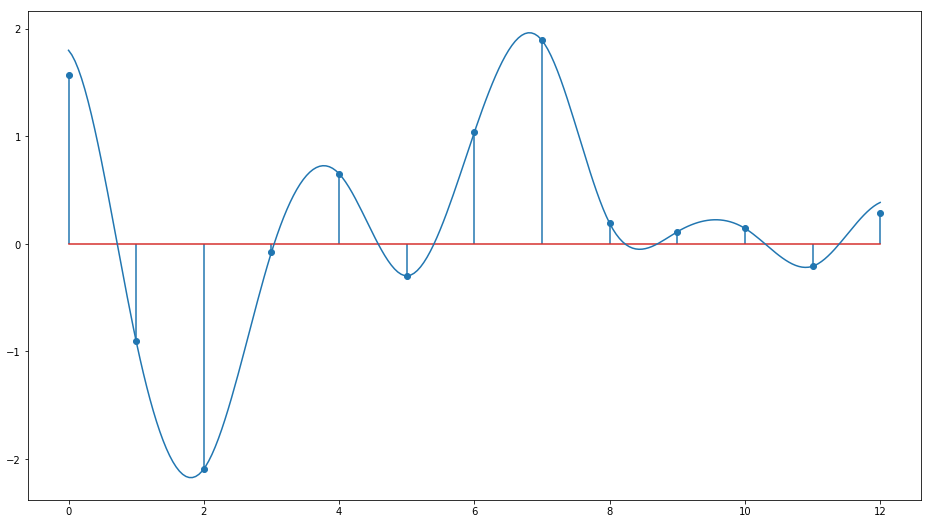
\includegraphics[width=0.9\textwidth]{img/bsplines/interpol.png}
    \caption{Kubische B-Spline-Interpolation f\"ur Abtastung an den Werten $n = 0, \dots, 12$.}\label{bsplines_interpol_pic}
\end{figure}
%
%
%
\subsubsection{Verbindung zur Nyquist-Sampling-Theorie}
%
%
Wir wollen als Abschluss eine Verbindung zum Sampling und der Interpolation~\cite[Kapitel~6.1]{proakis2013} von bandbegrenzten Funktionen mit endlicher Energie ziehen. Nehmen wir als Wiederholung zun\"achst an, dass das bandbegrenzte Signal $x_a$ mit endlicher Energie und Fourier-Transformation $X_a$ mindestens kritisch mit Rate $F_s$ zu den Werten $x[n]$ abgetastet wurde. Wir bezeichnen mit $X$ die \gls{dtft} von $x[n]$. Dann gilt als Zusammenhang zwischen den beiden Spektra, dass
\begin{equation}
    X(f) = F_s \Sum{k=-\infty}{+\infty}{
        X_a((f - k) F_s)
    } ,
\end{equation}
was die Periodifizierung des Frequenzbereiches nach Abtastung ausdr\"uckt. Nach Annahme der kritischen Abtastung findet hier kein Aliasing statt, sodass f\u"r $f \in [-F_s/2,+F_s/2]$ gilt, dass $F_s \cdot X_a(f) = X(f)$. Au{\ss}erdem k\"onnen wir das Spektrum der abgetasteten Werte $X$ durch
\begin{equation}
    X(f) = \Sum{n=-\infty}{+\infty}{x[n] \exp(- \jmath 2 \pi f n / F_s)}
\end{equation}
ausdr\"ucken k\"onnen. Nun k\"onnen wir das analoge Signal $x_a$ in Abh\"angigkeit von den Abtastwerten darstellen. Es gilt mit $T = 1/F_s$, dass
\begin{align*}
    x_a(t) &= \Int{-F_s/2}{+F_s/2}{
        X_a(f) \exp(\jmath 2 \pi f t)
    }{f} = \frac{1}{F_s} \Int{-F_s/2}{+F_s/2}{
        \left(
            \Sum{n=-\infty}{+\infty}{x[n] \exp(- \jmath 2 \pi f n / F_s)}
        \right) \exp(\jmath 2 \pi f t)
    }{f} \\
    &= \frac{1}{F_s} 
        \Sum{n=-\infty}{+\infty}{
            x[n] \Int{-F_s/2}{+F_s/2}{\exp(- \jmath 2 \pi f n / F_s) \exp(\jmath 2 \pi f t)}{f}
        } \\
    &= \frac{1}{F_s} 
    \Sum{n=-\infty}{+\infty}{
        x[n] \Int{-F_s/2}{+F_s/2}{\exp(\jmath 2 \pi f (t - n/F_s))}{f}
    } 
    = \Sum{n=-\infty}{+\infty}{
        x[n] \frac{\sin(\pi(t-nT)/T)}{\pi(t-nT)/T}
    }.
\end{align*}
Das hei{\ss}t, dass die Funktion $g: \R \rightarrow \R$ mit
\begin{equation}\label{bsplines_sinckernel}
    g(t) = \frac{\sin(\pi t / T)}{(\pi t/T)}
\end{equation}
als \emph{Interpolations-Kernel} von bandbegrenzten und abgetasteten Funktionen betrachtet werden kann. Siehe \cref{eadf-interpol} f\"ur eine Anwendung dieser Art der Interpolation.

Nun k\"onnen wir eine analoge Rechnung f\"ur die B-Splines durchf\"uhren, indem wir einen Filter $b^{-1}[k]$ als inverse $Z$-Transformation von $1/B(z)$ aus \eqref{bsplines_ztrafo} definieren. Dann gilt
\begin{equation}
    c[k] = (b^{-1} \ast x)[k],
\end{equation}
was wir in \eqref{bsplines_interpol} einsetzen und dann
\begin{equation}
    s(t) = \Sum{n \in \Z}{}{
        (b^{-1} \ast x)[n] \beta^{\ell}(t - n)
    } = \Sum{n \in \Z}{}{
        x[n] \Sum{p \in \Z}{}{
            b^{-1,\ell}[p] \beta^{\ell}(t - n - p)
        }
    } = \Sum{n \in \Z}{}{
        x[n] h^\ell(t - n)
    }
\end{equation}
erhalten, wobei wir analog zu \eqref{bsplines_sinckernel} den Interpolationskernel $h: \R \rightarrow \R$ durch
\begin{equation}\label{bsplines_kernel}
    h^\ell(t) = \Sum{p \in \Z}{}{
        b^{-1,\ell}[p] \beta^{\ell}(t - p)
    }
\end{equation}
definiert haben. Man kann zeigen, dass $\lim_{l \rightarrow \infty} h^\ell = g$. Das hei{\ss}t, dass die $\Sinc$-Interpolation als Grenzwert der B-Spline Interpolation aufgefasst werden kann -- oder andersherum die B-Spline-Interpolation als Approximation der $\Sinc$-Interpolation. Das hei{\ss}t, dass auch im Frequenzbereich Konvergenz in der Form
\begin{equation}
    H^\ell(\omega) = \left(\frac{\sin(\omega/2)}{\omega/2}\right)^{\ell+1} \frac{1}{B^{\ell}(\exp(\jmath \omega))} \rightarrow_{\ell \rightarrow \infty} \Rect(\omega)
\end{equation} 
gegeben sein muss.

Zusammenfassend kann man sagen, dass B-Splines einen alternativen Zugang zu digitaler Signalverarbeitung bieten, welcher eng mit dem des Nyquist-Samplings verkn\"upft ist und als Approximation von diesem gesehen werden kann. B-Splines sind wegen ihrer effizienten und stabilen Implementierung sowohl bei der Analyse \eqref{bsplines_filter}, als auch der Synthese \eqref{bsplines_summation} vor allem f\"ur hochdimensionale Interpolationen sehr interessant.
